% Provenance (never printed): see sources/outline_sources.md (Year 1: field
% notebook, compass-clinometer, hand lens, sampling, polarising microscope and
% thin sections, safety). The readings of the Varden east limb are simulated
% in figdata/bachelor-1/attitude_stats.py (seed 83, errors of 3 degrees);
% problem values in the Book 3 scratch calculator calc/ch06.py.
\chapter{क्षेत्र और प्रयोगशाला विधियाँ I}\label{ch:b1:field-lab-methods-1}

वार्डन पहाड़ियों का मानचित्रण करने वाली एक भूवैज्ञानिक अपने साथ बहुत कम ले जाती है: एक नोटबुक, एक पेंसिल, एक
उपग्रह रिसीवर, एक कंपास-क्लिनोमीटर, एक हाथ-लेंस और कुछ नमूना-थैलियाँ। इनसे वह तय करती है कि वह कहाँ खड़ी है,
परतों के \omterm{def:b1:geological-maps:attitude}{नति} मापती है, चट्टानों के नाम रखती है, और वे नमूने वापस लाती है जिन्हें प्रयोगशाला काटेगी, पीसेगी और
सूक्ष्मदर्शी से देखेगी। पिछले अध्यायों की हर संख्या --- मानचित्र पर एक \omterm{def:b1:geological-maps:attitude}{अभिविन्यास}, एक काट में एक \omterm{def:b1:geological-maps:attitude}{नति} ---
इसी प्रकार के पाठ से शुरू हुई थी, अपनी त्रुटि के साथ। यह अध्याय बताता है कि पेशेवर ये प्रेक्षण कैसे लेते हैं,
बार-बार के पाठों का औसत कैसे निकाला जाता है, और उनके प्रकीर्णन को एक अनिश्चितता में कैसे बदला जाता है। यह
वार्डन \omterm{def:b1:geological-maps:fold}{अपनति} की पूर्वी भुजा पर एक मौसम के पाठों के साथ समाप्त होता है।

\begin{recall}
किसी समतल का \omterm{def:b1:geological-maps:attitude}{अभिविन्यास} \omterm{def:b1:geological-maps:attitude}{नति-दिशा}/\omterm{def:b1:geological-maps:attitude}{नति} के रूप में लिखा जाता है, जैसे $081/12$, या दाएँ-हाथ के नियम से \omterm{def:b1:geological-maps:attitude}{स्ट्राइक}
और \omterm{def:b1:geological-maps:attitude}{नति} के रूप में (\cref{ch:b1:geological-maps})। चुंबकीय विचलन भौगोलिक उत्तर और उस दिशा के बीच का कोण है जिसमें
दिक्सूचक की सुई इंगित करती है (भौतिकी, कक्षा 11)। खनिज हाथ में उनकी चमक, विदलन, कठोरता और रंग से पहचाने
जाते हैं (पुस्तक 2, कक्षा 11)। संख्याओं के एक समुच्चय का माध्य और मानक विचलन उनके केंद्र और प्रकीर्णन का सार
देते हैं (गणित)।
\end{recall}

\section{नोटबुक और मानचित्र}

\begin{definition}[क्षेत्र-स्टेशन, क्षेत्र नोटबुक]\label{def:b1:field-lab-methods-1:station}
एक \emph{क्षेत्र-स्टेशन}\index{क्षेत्र-स्टेशन} एक क्रमांकित स्थान है जहाँ भूवैज्ञानिक प्रेक्षण करती है और उन्हें
दर्ज करती है: उसकी स्थिति, देखी गई चट्टानें, उनका \omterm{def:b1:geological-maps:attitude}{अभिविन्यास} और लिए गए नमूने। \emph{क्षेत्र नोटबुक}\index{क्षेत्र नोटबुक}
स्टेशनों का बँधा हुआ अभिलेख है, उसी क्रम में जिसमें वे देखे गए, उनके क्रमांकों, रेखाचित्रों और मापनों के साथ,
जो मौके पर ही लिखे जाते हैं।
\end{definition}

नोटबुक प्राथमिक अभिलेख है: जो स्टेशन पर नहीं लिखा गया, वह खो जाता है, और शाम को बना मानचित्र बस उन नोटों जितना
ही अच्छा होता है जिनके आधार पर वह बना। हर स्टेशन का एक क्रमांक होता है जो क्षेत्र-मानचित्र पर, नोटबुक में और वहाँ
लिए गए हर नमूना-थैली पर आता है। एक रेखाचित्र वह दिखाता है जो संख्याओं की सूची नहीं दिखा सकती ---
दो इकाइयाँ कैसे मिलती हैं, छोटी परतें किस ओर हैं, मुड़ी सतह पर पाठ कहाँ लिया गया --- और अपना पैमाना और
\omterm{def:b1:geological-maps:attitude}{अभिविन्यास} दर्ज करता है। तथ्य और व्याख्या अलग रखे जाते हैं: ``शेल पर चूना-पत्थर, \omterm{def:b1:geological-maps:geological-map}{संपर्क} तीखा'' एक प्रेक्षण है;
``\omterm{def:b1:cross-sections:unconformity}{असंगति}'' एक अनुमान है, और उसे उसी रूप में लिखा जाता है।

\begin{inthefield}[मानचित्रण का एक दिन]
% ledger: gps:smartphone-accuracy, gps:high-end
\begin{minipage}[t]{0.58\linewidth}\vspace{0pt}
एक मानचित्रण करने वाली भूवैज्ञानिक स्तर को आर-पार पार करने वाला एक मार्ग इस प्रकार योजित करती है कि वह हर इकाई से
बारी-बारी मिले, और जहाँ भी कोई \omterm{def:b1:geological-maps:geological-map}{संपर्क}, चट्टान का बदलाव या मापने योग्य सतह दिखे, वहाँ रुकती है। हर स्टेशन पर
वह स्टेशन का क्रमांक और स्थिति लिखती है, जो वह देखती है उसका रेखाचित्र बनाती है, \omterm{def:b1:geological-maps:attitude}{अभिविन्यास} मापती है, और
नमूने नोट करती है। स्थितियाँ एक उपग्रह रिसीवर से आती हैं: एक सामान्य रिसीवर, जैसे स्मार्टफ़ोन का, खुले आकाश
के नीचे आम तौर पर लगभग \qty{4.9}{m} के भीतर सटीक होता है, चट्टानों और पेड़ों के पास और खराब, जबकि दो आवृत्तियों
या सुधार सेवाओं वाले सर्वेक्षण रिसीवर कुछ सेंटीमीटर तक पहुँचते हैं। 1:10\,000 के मानचित्र पैमाने पर
\qty{4.9}{m} आधा मिलीमीटर है: एक सामान्य रिसीवर मानचित्रण के लिए पर्याप्त है, पर ज़मीन की धीमी गति मापने के लिए
नहीं (\cref{ch:b1:plate-kinematics})।
\end{minipage}\hfill
\begin{minipage}[t]{0.39\linewidth}\vspace{0pt}
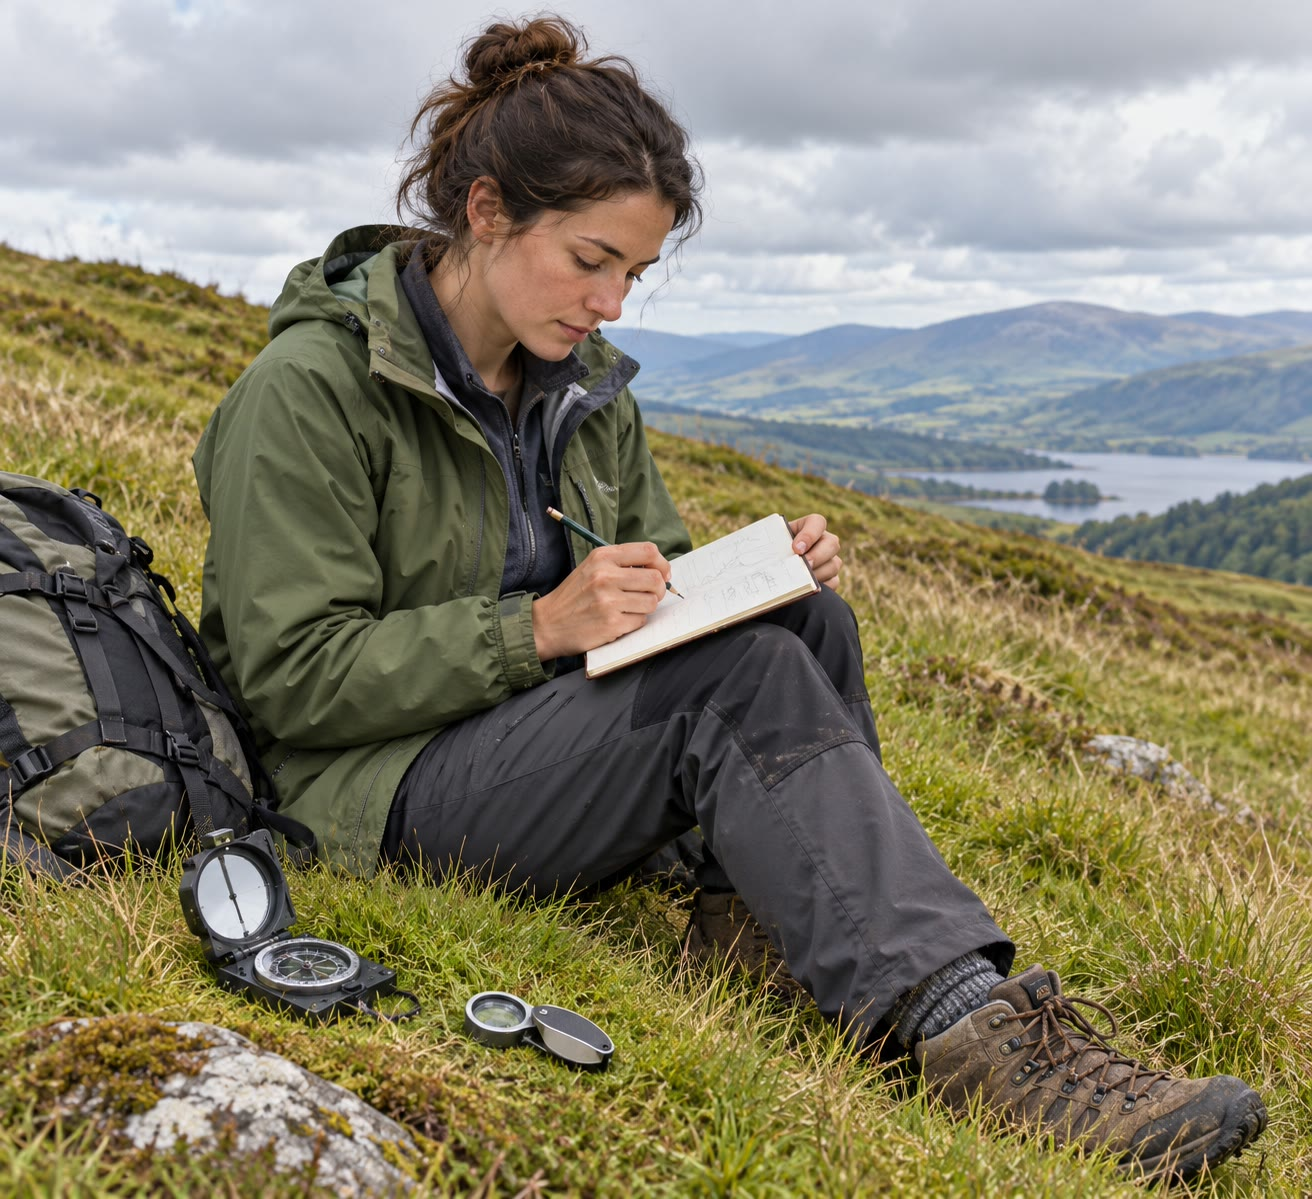
\includegraphics[width=\linewidth]{images/book3/ai/b1-field-notebook.jpg}
\end{minipage}
\end{inthefield}

\section{अभिविन्यासों का मापन}

किसी समतल का \omterm{def:b1:geological-maps:attitude}{अभिविन्यास} --- एक परत, एक भ्रंश, एक जोड़ --- कंपास-क्लिनोमीटर से मापा जाता है: \omterm{def:b1:field-lab-methods-1:trend-plunge}{दिगंश} पढ़ने के लिए
एक चुंबकीय दिक्सूचक, और क्षैतिज से कोण पढ़ने के लिए एक लोलक या स्तर। \omterm{def:b1:geological-maps:attitude}{स्ट्राइक} पढ़ने के लिए उसका किनारा सतह के
\omterm{def:b1:geological-maps:attitude}{स्ट्राइक} के अनुदिश रखा जाता है, या \omterm{def:b1:geological-maps:attitude}{नति} पढ़ने के लिए यंत्र को सतह पर उसकी सबसे खड़ी रेखा के अनुदिश रखा जाता है,
और उस रेखा के \omterm{def:b1:field-lab-methods-1:trend-plunge}{दिगंश} से \omterm{def:b1:geological-maps:attitude}{नति-दिशा}।

\begin{omfigure}
\begin{tikzpicture}[font=\scriptsize]
% (a) plan view
\begin{scope}
\fill[icsJurassic!25] (0,0) -- (3.6,0.5) -- (3.9,2.9) -- (0.3,2.4) -- cycle;
\draw (0,0) -- (3.6,0.5) -- (3.9,2.9) -- (0.3,2.4) -- cycle;
\draw[omDef, thick] (0.4,1.55) -- (3.5,1.98);
\node[omDef, above, rotate=8, fill=icsJurassic!25, inner sep=1pt] at (0.95,1.65) {स्ट्राइक रेखा};
% compass box laid along the strike line
\begin{scope}[shift={(2.5,1.84)}, rotate=8]
\draw[fill=white] (-0.6,0) rectangle (0.6,0.32);
\draw (0,0.16) circle (0.12);
\end{scope}
\draw[omThm, thick, -{Stealth[length=2mm]}] (1.6,1.71) -- (1.75,0.62);
\node[omThm, right, fill=icsJurassic!25, inner sep=1pt] at (1.78,0.85) {नति-दिशा};
\node[below, align=center] at (1.95,-0.15) {(क) योजना दृश्य: कंपास का किनारा\\ स्ट्राइक के अनुदिश};
\draw[->] (4.3,1.6) -- (4.3,2.4) node[above] {\omnameCompassN};
\end{scope}
% (b) side view, vertical section along the dip direction
\begin{scope}[xshift=5.8cm]
\fill[icsJurassic!25] (0,1.6) -- (3.6,0.2) -- (3.6,-0.3) -- (0,-0.3) -- cycle;
\draw[thick] (0,1.6) -- (3.6,0.2);
% clinometer resting on the surface
\begin{scope}[shift={(2.5,0.6278)}, rotate=-21.25]
\draw[fill=white] (-0.75,0) rectangle (0.75,0.3);
\draw (0,0.15) circle (0.11);
\draw[black!70] (0,0.15) -- ++(-68.75:0.11);
\end{scope}
% dip angle at the lower end of the surface
\coordinate (P) at (0.7,1.3278);
\draw[black!60] (P) -- ++(1.6,0) node[right] {क्षैतिज};
\draw[omThm] ($(P)+(1.1,0)$) arc[start angle=0, end angle=-21.25, radius=1.1];
\node[omThm] at ($(P)+(0.9,-0.15)$) {$\delta$};
\node[below, align=center] at (1.8,-0.35) {(ख) नति-दिशा के अनुदिश काट: सबसे खड़ी रेखा पर क्लिनोमीटर};
\end{scope}
\end{tikzpicture}

{\small \omterm{def:b1:geological-maps:attitude}{अभिविन्यास} का मापन (योजनाबद्ध)। (क) परत पर क्षैतिज रखे कंपास का किनारा \omterm{def:b1:geological-maps:attitude}{स्ट्राइक} देता है; \omterm{def:b1:geological-maps:attitude}{नति-दिशा} उसके
लंबवत, परत के नीचे की ओर है। (ख) सबसे खड़ी रेखा के अनुदिश उसके किनारे पर रखा क्लिनोमीटर \omterm{def:b1:geological-maps:attitude}{नति} $\delta$ देता है।}
\end{omfigure}

किसी रेखा --- एक \omterm{def:b1:geological-maps:fold}{वलन-अक्ष}, भ्रंश-सतह पर एक खरोंच, कंकड़ का लंबा अक्ष --- की अपनी दिशा होती है।

\begin{definition}[दिगंश और नमन]\label{def:b1:field-lab-methods-1:trend-plunge}
किसी रेखा का \emph{दिगंश}\index{दिगंश (रेखा का)} उसके क्षैतिज प्रक्षेप का दिगंश है, जो रेखा के उस सिरे की ओर
मापा जाता है जो नीचे की ओर इंगित करता है। उसका \emph{नमन}\index{नमन} रेखा और क्षैतिज के बीच का कोण है, जो उस
ऊर्ध्वाधर तल में मापा जाता है जिसमें वह है। \ang{015} की ओर \ang{20} नमन करने वाली रेखा $20\to015$ लिखी जाती है।
\end{definition}

\omterm{def:b1:field-lab-methods-1:trend-plunge}{दिगंश} $t$ और \omterm{def:b1:field-lab-methods-1:trend-plunge}{नमन} $p$ वाली एक रेखा का नीचे की ओर इकाई सदिश, पूर्व, उत्तर और ऊपर घटकों में, इस प्रकार लिखा जाता है:
$(\cos p\sin t, \cos p\cos t, -\sin p)$ है; \omterm{def:b1:geological-maps:attitude}{नति-दिशा} $\alpha$ और \omterm{def:b1:geological-maps:attitude}{नति} $\delta$ वाले समतल में पड़ी रेखा, \omterm{def:b1:field-lab-methods-1:trend-plunge}{दिगंश} $t$ के
ऊर्ध्वाधर तल में उस समतल की \omterm{def:b1:cross-sections:apparent-dip}{आभासी नति} जितनी नमित होती है, अतः $\tan p = \tan\delta\cos(\alpha - t)$
(\cref{thm:b1:cross-sections:apparent-dip})।

\subsection{चुंबकीय विचलन}

दिक्सूचक की सुई चुंबकीय उत्तर की ओर इंगित करती है, भौगोलिक उत्तर की ओर नहीं; दोनों के बीच का कोण चुंबकीय
विचलन है, जो धनात्मक गिना जाता है जब चुंबकीय उत्तर भौगोलिक उत्तर के पूर्व में हो। इस पुस्तक के मानचित्र और
\omterm{def:b1:geological-maps:attitude}{अभिविन्यास} भौगोलिक दिगंशों का उपयोग करते हैं।

\begin{method}[दिक्सूचक दिगंश का सुधार]\label{met:b1:field-lab-methods-1:declination}
\begin{enumerate}
  \item स्थान और तिथि के लिए चुंबकीय विचलन $D$ पृथ्वी के क्षेत्र के एक प्रतिरूप से ज्ञात कीजिए (पूर्व धनात्मक, पश्चिम ऋणात्मक)।
  \item दिक्सूचक पर पढ़े गए हर \omterm{def:b1:field-lab-methods-1:trend-plunge}{दिगंश} में उसे जोड़िए: भौगोलिक \omterm{def:b1:field-lab-methods-1:trend-plunge}{दिगंश} $=$ चुंबकीय \omterm{def:b1:field-lab-methods-1:trend-plunge}{दिगंश} $+ D$, \ang{360} के मॉड्यूलो।
  \item नतियों और नमनों को छोड़ दीजिए: वे क्षैतिज से गुरुत्व के साथ मापे जाते हैं, सुई से नहीं।
\end{enumerate}
अधिकांश क्षेत्र-दिक्सूचकों को $D$ यांत्रिक रूप से जोड़ने के लिए सेट किया जा सकता है; सेटिंग, और वह वर्ष जिसके लिए
वह बनाई गई थी, नोटबुक में लिखे जाते हैं।
\end{method}

\begin{dated}{2026}
% ledger: noaa:wmm-edinburgh, noaa:wmm-reykjavik, noaa:wmm-anchorage, noaa:wmm-wellington
1 जनवरी 2026 को विश्व चुंबकीय मॉडल (संस्करण 2025) एडिनबरा पर चुंबकीय विचलन \ang{-0.47} (पश्चिम) देता है, जो
हर वर्ष \ang{+0.20} बदलता है; रेक्याविक पर \ang{-11.28}, जो हर वर्ष \ang{+0.30} बदलता है; एंकरेज पर
\ang{+14.20} (पूर्व), जो हर वर्ष \ang{-0.28} बदलता है; और वेलिंगटन पर \ang{+23.23}। जो भूवैज्ञानिक वेलिंगटन में सुधार
भूल जाए, वह हर \omterm{def:b1:field-lab-methods-1:trend-plunge}{दिगंश} को \ang{23} से अधिक गलत जगह रखेगी; जो दस वर्ष पहले की एडिनबरा की सेटिंग दोबारा प्रयोग
करे, उसमें लगभग \ang{2} की त्रुटि आएगी।
\end{dated}

\subsection{बार-बार के पाठ}
एक शय्या-तल के एक पाठ में त्रुटियाँ होती हैं: सतह कभी पूर्ण समतल नहीं होती, यंत्र पूरी तरह सेट नहीं होता, और पाठ
एक अंश तक पूर्णांकित होता है। इसलिए भूवैज्ञानिक वही सतह कई बार मापती है, या एक ही भुजा की कई सतहें, और औसत
निकालती है। दिगंशों का औसत सावधानी माँगता है: पाठ \ang{355} और \ang{005} ऐसी दिशाओं का वर्णन करते हैं जो
\ang{10} दूर हैं, पर उनका अंकगणितीय माध्य, \ang{180}, विपरीत दिशा की ओर इंगित करता है। सही माध्य सदिशों से काम
करता है।

\begin{definition}[औसत अभिविन्यास (सदिश माध्य)]\label{def:b1:field-lab-methods-1:mean-orientation}
\omterm{def:b1:geological-maps:attitude}{नति-दिशा} $\alpha$ और \omterm{def:b1:geological-maps:attitude}{नति} $\delta$ वाले एक समतल के लिए, मान लीजिए
\[
  \vec n = (\sin\delta\sin\alpha,\ \sin\delta\cos\alpha,\ \cos\delta)
\]
पूर्व, उत्तर और ऊपर घटकों में उसका ऊर्ध्वमुखी इकाई अभिलंब है। $N$ पाठों के अभिलंबों $\vec n_1, \dots, \vec n_N$ का
\emph{औसत अभिविन्यास}\index{औसत अभिविन्यास} (या \emph{सदिश माध्य}) वह समतल है जिसका अभिलंब
$\vec m = \vec S/\|\vec S\|$ है, जहाँ $\vec S = \sum_i \vec n_i$ उनका परिणामी है; $\bar R = \|\vec S\|/N$ \emph{औसत
परिणामी लंबाई} है। औसत \omterm{def:b1:geological-maps:attitude}{नति-दिशा} और \omterm{def:b1:geological-maps:attitude}{नति} $\bar\alpha = \operatorname{atan2}(S_E, S_N)$ और
$\bar\delta = \arccos(S_U/\|\vec S\|)$ हैं।
\end{definition}

यह कि $\vec n$ अभिलंब है, \cref{ch:b1:geological-maps} से निकलता है: समतल $z = -\tan\delta\,(x\sin\alpha + y\cos\alpha)$
का ऊर्ध्वमुखी अभिलंब $(\tan\delta\sin\alpha, \tan\delta\cos\alpha, 1)$ है, जिसकी लंबाई $1/\cos\delta$ है।

\begin{proposition}[सदिश माध्य सबसे निकटतम दिशा है]\label{prop:b1:field-lab-methods-1:vector-mean}
सभी इकाई सदिशों $\vec u$ में, औसत अभिलंब $\vec m$ $\sum_i \vec n_i\cdot\vec u = \sum_i \cos\theta_i(\vec u)$ को
अधिकतम करता है, जहाँ $\theta_i(\vec u)$, $\vec n_i$ और $\vec u$ के बीच का कोण है; समतुल्य रूप से, वह
$\sum_i \|\vec n_i - \vec u\|^2$ को न्यूनतम करता है। इसके अतिरिक्त
\[
  \bar R = \frac1N\sum_i \cos\theta_i, \qquad \theta_i = \theta_i(\vec m),
\]
अतः $0 < \bar R \le 1$ है, जिसमें $\bar R = 1$ केवल तब जब सारे पाठ मेल खाएँ, और, जब प्रकीर्णन छोटा हो, तब पाठों
और उनके माध्य के बीच का वर्ग-माध्य-मूल कोण
\[
  \theta_{\text{वर्ग-माध्य-मूल}} \approx \sqrt{2(1 - \bar R)} \quad\text{(रेडियन में)}.
\]
\end{proposition}

\begin{proof}
$\sum_i \vec n_i\cdot\vec u = \vec S\cdot\vec u \le \|\vec S\|$ कोशी–श्वार्ज़ असमिका से, जो ठीक तब समता में है जब
$\vec u = \vec m$। चूँकि $\|\vec n_i - \vec u\|^2 = 2 - 2\,\vec n_i\cdot\vec u$, दोनों समस्याएँ एक ही हैं। $\vec u = \vec m$
पर सीमा प्राप्त होती है: $\|\vec S\| = \sum_i\cos\theta_i$, जो $\bar R$ का सूत्र है। अंत में
$\cos\theta \approx 1 - \theta^2/2$ छोटे $\theta$ के लिए, अतः $1 - \bar R \approx
\frac1N\sum_i\theta_i^2/2 = \theta_{\text{वर्ग-माध्य-मूल}}^2/2$।
\end{proof}

दो कोणों में त्रुटियाँ अभिलंब को कैसे हिलाती हैं? $\vec n$ का अवकलन करने पर,
\[
  \frac{\partial\vec n}{\partial\delta} = (\cos\delta\sin\alpha,\ \cos\delta\cos\alpha,\ -\sin\delta),
  \qquad
  \frac{\partial\vec n}{\partial\alpha} = (\sin\delta\cos\alpha,\ -\sin\delta\sin\alpha,\ 0):
\]
पहले की लंबाई 1 है, दूसरे की लंबाई $\sin\delta$ है, और दोनों लंबवत हैं। अतः छोटी त्रुटियाँ $\Delta\delta$ और
$\Delta\alpha$ अभिलंब को इस कोण से घुमाती हैं
\[
  \Delta\theta \approx \sqrt{\Delta\delta^2 + \sin^2\delta\,\Delta\alpha^2}.
\]
मंद \omterm{def:b1:geological-maps:attitude}{नति} वाली परत पर \omterm{def:b1:geological-maps:attitude}{नति-दिशा} की त्रुटि समतल को लगभग नहीं बदलती: \ang{12} \omterm{def:b1:geological-maps:attitude}{नति} वाली परत पर \ang{3} की \omterm{def:b1:geological-maps:attitude}{नति-दिशा}
त्रुटि समतल को केवल $3\sin\ang{12} = \ang{0.6}$ घुमाती है। इसका विलोम भूवैज्ञानिक की कठिनाई है: मंद परत की
\omterm{def:b1:geological-maps:attitude}{नति-दिशा} उसके समतल से ठीक-ठीक तय नहीं होती, और सतह के छोटे उभार उसे दूर तक बिखेर देते हैं। $N$ स्वतंत्र पाठों के माध्य की, जिनका मानक विचलन $s$ है, मानक त्रुटि
$s/\sqrt N$ है (गणित): उसे आधा करने के लिए चार गुना अधिक पाठ
चाहिए।

\begin{omfigure}
\begin{tikzpicture}
\begin{axis}[name=dd, width=0.47\linewidth, height=4.6cm, ybar, bar width=0.8,
  xmin=72.5, xmax=88.5, ymin=0, ymax=8.5, ytick={0,2,4,6,8},
  tick label style={font=\scriptsize}, label style={font=\small},
  xlabel={नति-दिशा (\si{\degree})}, ylabel={पाठ}]
\addplot[fill=icsJurassic!40, draw=black] table[x=value, y=count] {figdata/out/bachelor-1-attitude_stats-hist-dd.dat};
\draw[omThm, thick] (axis cs:80.84,0) -- (axis cs:80.84,8.5);
\draw[omThm, densely dashed] (axis cs:77.91,0) -- (axis cs:77.91,8.5);
\draw[omThm, densely dashed] (axis cs:83.77,0) -- (axis cs:83.77,8.5);
\end{axis}
\begin{axis}[at={(dd.east)}, anchor=west, xshift=1.1cm, width=0.47\linewidth, height=4.6cm,
  ybar, bar width=0.8, xmin=5.5, xmax=18.5, ymin=0, ymax=8.5, ytick={0,2,4,6,8},
  tick label style={font=\scriptsize}, label style={font=\small},
  xlabel={नति (\si{\degree})}]
\addplot[fill=icsJurassic!40, draw=black] table[x=value, y=count] {figdata/out/bachelor-1-attitude_stats-hist-dip.dat};
\draw[omThm, thick] (axis cs:12.36,0) -- (axis cs:12.36,8.5);
\draw[omThm, densely dashed] (axis cs:10.24,0) -- (axis cs:10.24,8.5);
\draw[omThm, densely dashed] (axis cs:14.48,0) -- (axis cs:14.48,8.5);
\end{axis}
\end{tikzpicture}

{\small वार्डन पूर्वी भुजा की शय्या के पच्चीस अनुकरणीय पाठ, जिनका मॉडल \omterm{def:b1:geological-maps:attitude}{अभिविन्यास} $080.7/12.2$ है, हर एक में दोनों
कोणों पर \ang{3} मानक विचलन की त्रुटियों के साथ, एक अंश तक पूर्णांकित। ठोस रेखा: माध्य; बिंदुरेखा: दोनों ओर एक
मानक विचलन ($080.8 \pm 2.9$ और $12.4 \pm 2.1$)। 25 पाठों का सदिश माध्य $080.9/12.3$ है।}
\end{omfigure}

\section{हाथ-लेंस और क्षेत्र में पहचान}

अधिकांश चट्टानों के नाम प्रयोगशाला के काम से पहले, क्षेत्र में रखे जाते हैं, उन खनिजों से जो हाथ-लेंस दिखाता है और
उस ढंग से जिससे चट्टान टूटती है। भूवैज्ञानिक एक ताज़ी सतह देखती है, क्योंकि अपक्षय चट्टान पर परत चढ़ाता और उसका
रंग बदलता है, और कणों का आकार नोट करती है (क्या वे नंगी आँख से दिखते हैं, लेंस से, या बिल्कुल नहीं), उनके
आकार, क्या वे मोज़ेक की तरह एक-दूसरे में गुँथे हैं या रेत की तरह सीमेंट से जुड़े हैं, और कोई संरेखण। खनिज उन
गुणों से पहचाने जाते हैं जो अध्याय के आरंभ में स्मरण किए गए: स्फटिक की काँच-जैसी चमक और विदलन का अभाव, फ़ेल्सपार
के दो विदलन और मंद सफ़ेदी, अभ्रक के पत्रक, कैल्साइट का समचतुर्भुजाकार विदलन। कठोरता एक इस्पात की नोक से परखी
जाती है: स्फटिक इस्पात से कठोर है और कैल्साइट कहीं नरम।

पेशेवर लोग तनु हाइड्रोक्लोरिक अम्ल की एक छोटी ड्रॉपर-बोतल रखते हैं: एक कार्बोनेट चट्टान उस स्थान पर कार्बन डाइऑक्साइड के बुलबुले
छोड़ती है जहाँ बूँद गिरती है (रसायन विज्ञान)। कैल्साइट तेज़ी से प्रतिक्रिया करता है; डोलोमाइट चूर्ण न हो तो मंद।
अम्ल दस्तानों और आँखों की सुरक्षा के साथ संभाला जाता है, और इस पुस्तक के किसी पाठक द्वारा कभी नहीं: यह विवरण पेशेवर
व्यवहार का है।

\section{नमूने}

\begin{definition}[अभिमुखित नमूना]\label{def:b1:field-lab-methods-1:sample}
एक \emph{अभिमुखित नमूना}\index{अभिमुखित नमूना} वह चट्टान का नमूना है जिस पर भूवैज्ञानिक ने उसे हटाने से पहले उसकी
एक सतह का \omterm{def:b1:geological-maps:attitude}{अभिविन्यास} अंकित कर लिया है (एक \omterm{def:b1:geological-maps:attitude}{स्ट्राइक} रेखा और एक नति-तीर, या एक रेखा का \omterm{def:b1:field-lab-methods-1:trend-plunge}{दिगंश}), ताकि नमूना
प्रयोगशाला में उसकी क्षेत्र-स्थिति में वापस रखा जा सके।
\end{definition}

एक नमूना तभी उपयोगी है जब वह उस इकाई का प्रतिनिधि हो जिसका वह प्रतिनिधित्व करता है --- ताज़ा, अपक्षयित नहीं,
किसी शिरा या गिरे हुए खंड से नहीं लिया गया --- और जब उसका स्रोत निश्चित हो। हर एक को स्टेशन का क्रमांक और एक
नमूना-क्रमांक मिलता है, जो चट्टान पर और थैली पर लिखा जाता है, और नोटबुक में उसकी स्थिति, उसकी इकाई और उसे लेने
के कारण के साथ सूचीबद्ध होता है। रासायनिक या समस्थानिक विश्लेषण के नमूने, जिनके परिणाम दशकों बाद प्रकाशित हो सकते
हैं, मैदान से प्रयोगशाला तक एक लिखित अभिलेख के द्वारा हर उस हाथ के साथ ट्रैक किए जाते हैं जिससे वे गुज़रते हैं ---
एक अभिरक्षा-शृंखला --- ताकि इसमें कोई संदेह न रहे कि किस चट्टान ने कौन-सा अंक दिया। अभिमुखित नमूने तब चाहिए
जब चट्टान के भीतर किसी चीज़ की दिशा मायने रखे: खनिजों का संरेखण, सूक्ष्मदर्शी में दिखने वाली संरचना, या वह
चुंबकन की दिशा जो चट्टान बनते समय प्राप्त करती है।

\section{पतली काटें और ध्रुवण सूक्ष्मदर्शी}

\begin{definition}[पतली काट]\label{def:b1:field-lab-methods-1:thin-section}
एक \emph{पतली काट}\index{पतली काट} चट्टान का एक टुकड़ा है, जो एक काँच की स्लाइड पर चिपकाया गया और
\qty{30}{\micro\metre} की मानक मोटाई तक पीसा गया है, इतना पतला कि अधिकांश खनिज प्रकाश को संचरित करें।
\end{definition}

\begin{inthelab}[पतली काट बनाना]
% ledger: jaic:thin-section, jaic:epoxy-ri
\begin{minipage}[t]{0.58\linewidth}\vspace{0pt}
प्रयोगशाला की तैयारी में एक तकनीशियन हीरे की आरी से नमूने का एक छोटा खंड काटता है, एक सतह को पूरी तरह समतल पीसता
है, और उसे एक काँच की स्लाइड पर एक इपॉक्सी रेज़िन से चिपकाता है जिसका अपवर्तनांक, 1.54 से 1.55, लगभग स्फटिक
जितना है। खंड का अधिकांश भाग तब आरी से अलग किया जाता है, और टुकड़े को एक घूमती पटिया पर अधिकाधिक बारीक
घर्षक के साथ तब तक घिसा जाता है जब तक वह \qty{30}{\micro\metre} मोटा न हो जाए। तकनीशियन सूक्ष्मदर्शी के नीचे
स्फटिक कणों के दिखाए रंगों से मोटाई जाँचता है (\cref{ch:b1:optical-mineralogy}), और एक पतले आवरण-काँच या एक
चमकाई सतह के साथ समाप्त करता है। छिद्रयुक्त या भुरभुरी चट्टानें पहले रेज़िन में भिगोई जाती हैं ताकि वे साथ
जुड़ी रहें।
\end{minipage}\hfill
\begin{minipage}[t]{0.39\linewidth}\vspace{0pt}
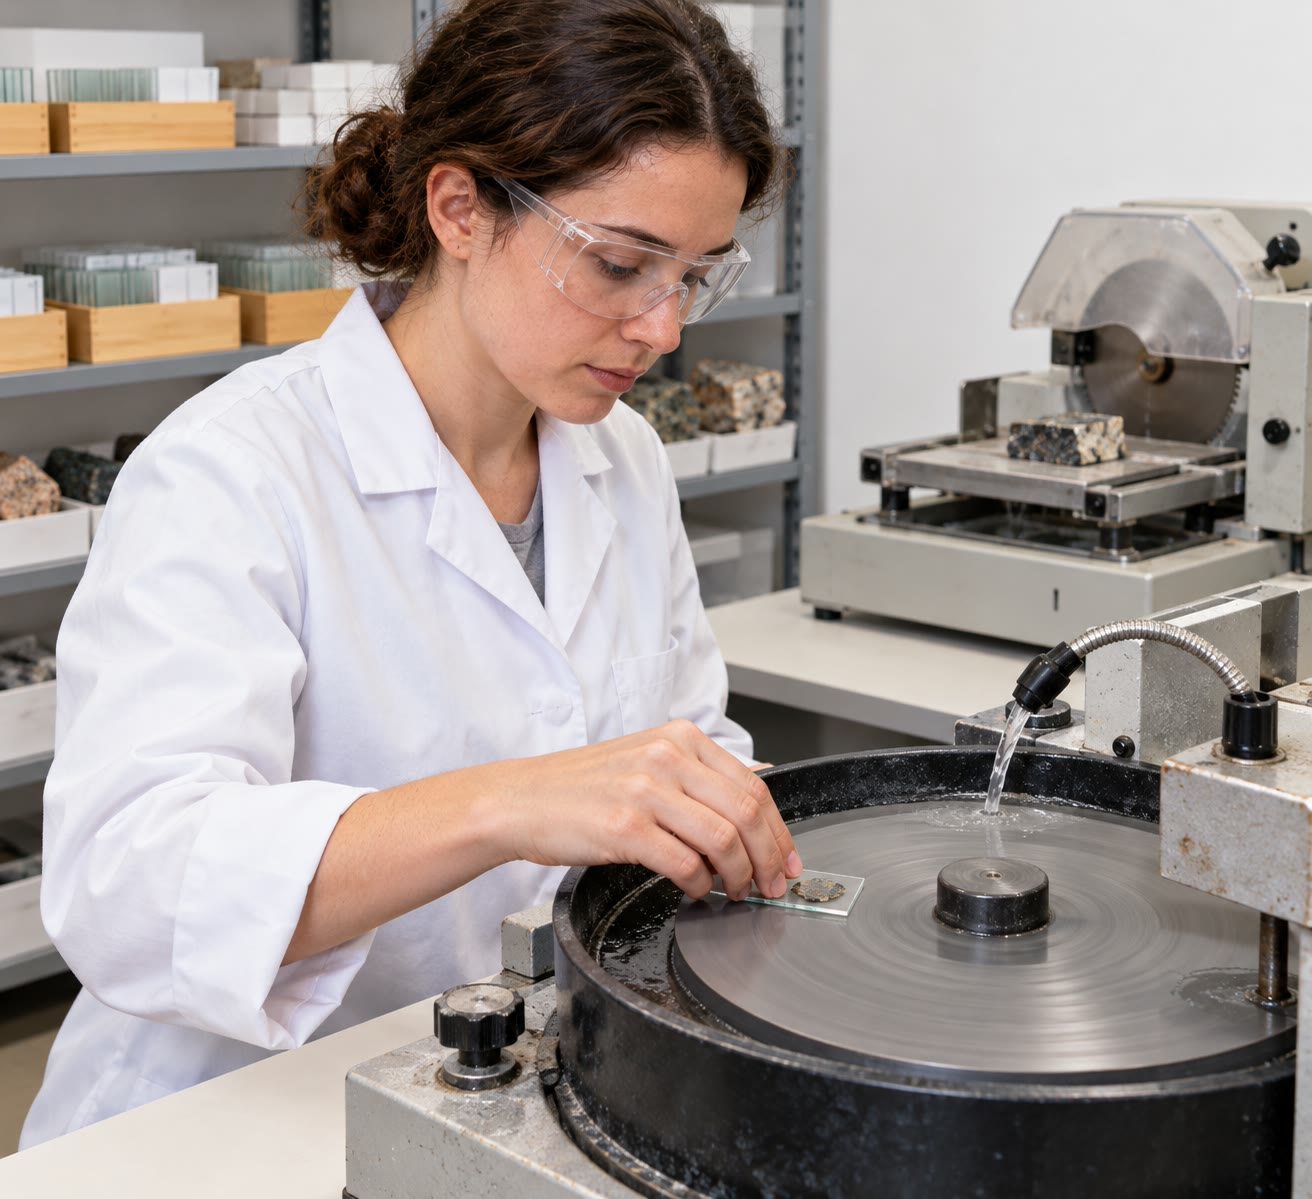
\includegraphics[width=\linewidth]{images/book3/ai/b1-thin-section-lab.jpg}
\end{minipage}
\end{inthelab}

\omterm{def:b1:field-lab-methods-1:thin-section}{पतली काट} एक ऐसे सूक्ष्मदर्शी से देखी जाती है जिसमें दो ध्रुवक फ़िल्टर लगे हैं। रैखिक ध्रुवण भौतिकी का विषय है: यहाँ
इतना पर्याप्त है कि एक ध्रुवक फ़िल्टर केवल एक दिशा में कंपित प्रकाश संचरित करता है, और समकोण पर रखे दो फ़िल्टर
कुछ भी संचरित नहीं करते।

\begin{definition}[ध्रुवण सूक्ष्मदर्शी, समतल-ध्रुवित प्रकाश, आड़े ध्रुवक]\label{def:b1:field-lab-methods-1:microscope}
एक \emph{ध्रुवण सूक्ष्मदर्शी}\index{ध्रुवण सूक्ष्मदर्शी} एक संचरित-प्रकाश सूक्ष्मदर्शी है, जिसके मंच के नीचे एक ध्रुवक
फ़िल्टर (ध्रुवक) है, और मंच \ang{360} घूमता है और अंशांकित पैमाने पर चलता है; और अभिदृश्यक तथा नेत्रिका के बीच
एक दूसरा ध्रुवक फ़िल्टर (विश्लेषक) है, जिसे प्रकाश-पथ में भीतर या बाहर किया जा सकता है, और जिसका कंपन-दिशा
ध्रुवक की कंपन-दिशा के समकोण पर है। विश्लेषक बाहर होने पर नमूना \emph{समतल-ध्रुवित प्रकाश}\index{समतल-ध्रुवित प्रकाश}
में दिखता है; भीतर होने पर वह \emph{आड़े ध्रुवकों}\index{आड़े ध्रुवक} के बीच दिखता है।
\end{definition}

\begin{omfigure}
\begin{tikzpicture}[font=\scriptsize, x=1cm, y=0.62cm]
\def\comp#1#2#3{\draw[fill=#3] (-1.1,#1-0.18) rectangle (1.1,#1+0.18); \node[right] at (1.3,#1) {#2};}
\draw[omThm!60, line width=3pt, -{Stealth[length=3mm]}] (0,0.3) -- (0,10.6);
\draw[fill=yellow!40] (0,0) circle (0.3); \node[right] at (1.3,0) {लैंप};
\comp{1.3}{ध्रुवक: एक कंपन-दिशा संचरित करता है}{omDef!25}
\draw[omDef, thick, <->] (-0.5,1.3) -- (0.5,1.3);
\draw[fill=white] (-1.0,2.3) .. controls (0,2.75) .. (1.0,2.3) .. controls (0,1.85) .. (-1.0,2.3);
\node[right] at (1.3,2.3) {संघनित्र};
\draw[fill=black!70] (-1.6,3.4) rectangle (1.6,3.55);
\draw[fill=icsJurassic!40] (-0.5,3.55) rectangle (0.5,3.65);
\node[right] at (1.7,3.48) {अंशांकित घूर्णी मंच, पतली काट के साथ};
\draw[fill=white] (-0.45,4.5) rectangle (0.45,5.4); \node[right] at (1.3,4.95) {अभिदृश्यक};
\comp{6.2}{सहायक स्लॉट}{black!10}
\comp{7.2}{विश्लेषक: अंदर (आड़े ध्रुवक) या बाहर (समतल-ध्रुवित प्रकाश)}{omDef!25}
\draw[omDef, thick, <->] (0,6.85) -- (0,7.55);
\comp{8.2}{बर्टरैंड लेंस (वैकल्पिक)}{black!5}
\draw[fill=white] (-0.35,9.1) rectangle (0.35,10.0); \node[right] at (1.3,9.55) {नेत्रिका, क्रॉस-तारों के साथ};
\end{tikzpicture}

{\small एक \omterm{def:b1:field-lab-methods-1:microscope}{ध्रुवण सूक्ष्मदर्शी} का प्रकाश-पथ (योजनाबद्ध, नीचे से ऊपर)। ध्रुवक और विश्लेषक समकोण पर कंपन करते हैं
(दोहरे तीर); उनके बीच कुछ न हो तो \omterm{def:b1:field-lab-methods-1:microscope}{आड़े ध्रुवक} एक काला क्षेत्र देते हैं।}
\end{omfigure}

\omterm{def:b1:field-lab-methods-1:microscope}{आड़े ध्रुवकों} के बीच, स्लाइड का काँच, इपॉक्सी और कोई भी समदैशिक खनिज (जिसके प्रकाशीय गुण हर दिशा में समान हों, जैसे
घनीय क्रिस्टलों में) मंच के घूर्णन से चाहे जैसे भी हो, काले रहते हैं। अधिकांश खनिज समदैशिक नहीं हैं: वे उनसे
गुज़रने वाले प्रकाश का ध्रुवण बदलते हैं, और व्यतिकरण वर्णों में दिखते हैं जो मंच के घूमने पर बदलते हैं और एक पूरे
चक्कर में चार बार लुप्त हो जाते हैं। वे ऐसा क्यों करते हैं, और रंग तथा कोण किसी खनिज की पहचान कैसे कराते हैं, यह
\cref{ch:b1:optical-mineralogy} का विषय है। \omterm{def:b1:field-lab-methods-1:thin-section}{पतली काट} में खनिज आम तौर पर लगभग $16\times$ से $400\times$ आवर्धन पर देखे जाते हैं।
% ledger: jaic:magnification

\begin{omfigure}
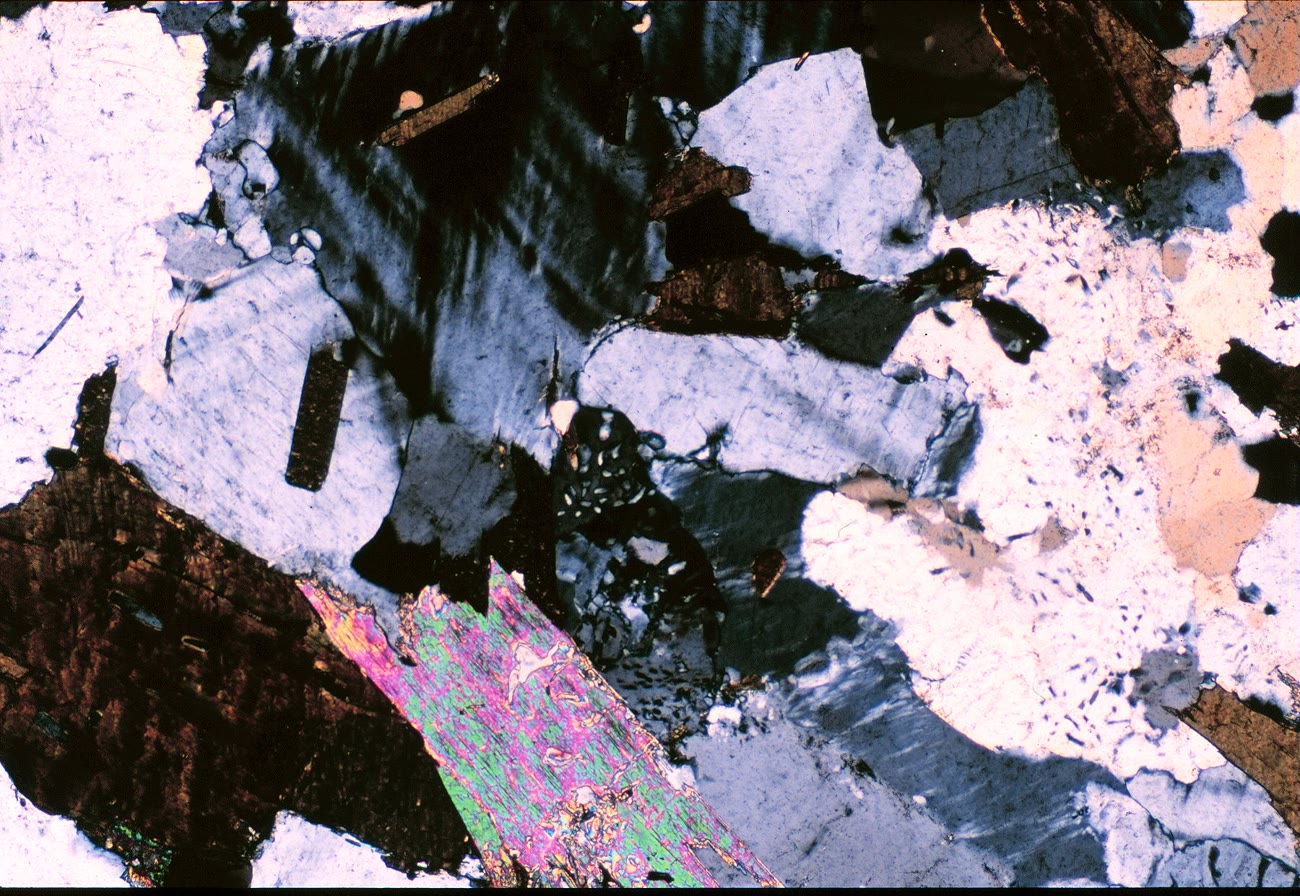
\includegraphics[width=0.55\linewidth]{images/book3/b1-granite-thin-section-xpl.jpg}
% ledger: commons:granite-xpl

{\small \omterm{def:b1:field-lab-methods-1:microscope}{आड़े ध्रुवकों} के बीच \omterm{def:b1:field-lab-methods-1:thin-section}{पतली काट} में एक ग्रेनाइट। बायोटाइट भूरा है, मस्कोवाइट चमकीले गुलाबी और हरे
व्यतिकरण-वर्ण दिखाता है, प्लैजियोक्लेज़ अपनी यमल-रचना से धारीदार है, और स्फटिक सफ़ेद से धूसर। फ़ोटो डार्ला
सोंड्रोल, CC0 (विकिमीडिया कॉमन्स)।}
\end{omfigure}

\begin{safety}
क्षेत्र और प्रयोगशाला का काम पेशेवर नियमों से सुरक्षित होता है, भाग्य से नहीं। क्षेत्र में भूवैज्ञानिक जोड़ों में
काम करते हैं या अपने मार्ग और लौटने के समय की लिखित योजना छोड़ जाते हैं; वे मौसम का पूर्वानुमान, मानचित्र और
प्राथमिक चिकित्सा साथ रखते हैं, चट्टानी ढलानों, खदान के मुखों के पैर और किनारे से दूर रहते हैं, और जहाँ चट्टान गिर
या टूट सकती है वहाँ हेलमेट और आँखों की सुरक्षा पहनते हैं; सक्रिय स्थलों पर कार्य संचालक के नियमों का पालन करता है।
प्रयोगशाला में आरियाँ और घूमती पटियाँ धूल कम रखने के लिए पानी के साथ सुरक्षा-आवरणों के पीछे चलती हैं, रेज़िन और
अम्ल दस्तानों और चश्मों के साथ, धुएँ-निष्कर्षण के नीचे संभाले जाते हैं, और हर रसायन का अपना सुरक्षा-डेटा पत्रक होता है।
इनमें से कोई गतिविधि अकेले इस पुस्तक के पाठक के लिए नहीं है: अध्याय पेशेवर व्यवहार का वर्णन करता है।
\end{safety}

\section{अभ्यास}

\begin{exercise}[$\star$]\label{exo:b1:field-lab-methods-1:1}
एक उपग्रह रिसीवर लगभग \qty{4.9}{m} के भीतर स्थितियाँ देता है। 1:10\,000 के मानचित्र पर वह कितना बड़ा है? 1:25\,000 पर?
\end{exercise}

\begin{exercise}[$\star$]\label{exo:b1:field-lab-methods-1:2}
बिना चुंबकीय विचलन सेटिंग वाला एक दिक्सूचक एक परत की \omterm{def:b1:geological-maps:attitude}{नति-दिशा} \ang{052} पढ़ता है। यदि पाठ 1 जनवरी 2026 को
रेक्याविक में लिया गया, तो भौगोलिक \omterm{def:b1:geological-maps:attitude}{नति-दिशा} दीजिए, फिर उसी दिन वेलिंगटन में (तिथि-बॉक्स)।
\end{exercise}

\begin{exercise}[$\star$]\label{exo:b1:field-lab-methods-1:3}
एक \omterm{def:b1:geological-maps:fold}{वलन-अक्ष} \ang{015} की ओर \ang{20} नमित है। उसका \omterm{def:b1:geological-maps:attitude}{अभिविन्यास} पाठ की तरह लिखिए और उसका नीचे की ओर इकाई सदिश
पूर्व, उत्तर और ऊपर घटकों में दीजिए।
\end{exercise}

\begin{exercise}[$\star$]\label{exo:b1:field-lab-methods-1:4}
एक ऊर्ध्वाधर जोड़ के तीन पाठ उसके अभिलंब के \omterm{def:b1:field-lab-methods-1:trend-plunge}{दिगंश} \ang{350}, \ang{358} और \ang{006} देते हैं। उनका अंकगणितीय माध्य
परिकलित कीजिए, फिर तीन क्षैतिज इकाई सदिशों के योग का \omterm{def:b1:field-lab-methods-1:trend-plunge}{दिगंश}। कौन-सा माध्य सही है?
\end{exercise}

\begin{exercise}[$\star\star$]\label{exo:b1:field-lab-methods-1:5}
एक ही परत की \omterm{def:b1:geological-maps:attitude}{नति} के पाँच पाठ \ang{34}, \ang{37}, \ang{35}, \ang{33} और \ang{36} हैं। उनका माध्य, उनका मानक विचलन
और माध्य की मानक त्रुटि परिकलित कीजिए।
\end{exercise}

\begin{exercise}[$\star\star$]\label{exo:b1:field-lab-methods-1:6}
एक भूवैज्ञानिक एक सममित \omterm{def:b1:geological-maps:fold}{वलन} की हर भुजा पर एक पाठ का औसत लेती है: $090/30$ और $270/30$। सदिश माध्य और $\bar R$
परिकलित कीजिए। क्या गड़बड़ हुआ है?
\end{exercise}

\begin{exercise}[$\star\star$]\label{exo:b1:field-lab-methods-1:7}
\omterm{def:b1:geological-maps:attitude}{अभिविन्यास} $080/12$ की एक शय्या-सतह पर खरोंचों का \omterm{def:b1:field-lab-methods-1:trend-plunge}{दिगंश} \ang{120} है। उनका \omterm{def:b1:field-lab-methods-1:trend-plunge}{नमन} क्या है? \omterm{def:b1:field-lab-methods-1:trend-plunge}{दिगंश} \ang{170} के लिए
वह क्या होगा?
\end{exercise}

\begin{exercise}[$\star\star$]\label{exo:b1:field-lab-methods-1:8}
एडिनबरा पर 1 जनवरी 2026 को चुंबकीय विचलन \ang{-0.47} है और हर वर्ष \ang{+0.20} बदलता है। यह मानते हुए कि बदलाव
स्थिर रहता है, वह कब शून्य तक पहुँचेगा, और 1 जनवरी 2030 को वह क्या होगा?
\end{exercise}

\begin{exercise}[$\star\star$]\label{exo:b1:field-lab-methods-1:9}
एक शय्या के तीन पाठ $080/10$, $080/12$ और $080/14$ हैं। दिखाइए कि उनका सदिश माध्य $080/12$ है, $\bar R$ और
$\sqrt{2(1 - \bar R)}$ परिकलित कीजिए, जो $\theta_{\text{वर्ग-माध्य-मूल}}$ का अनुमान है, और सटीक वर्ग-माध्य-मूल कोण से तुलना कीजिए।
\end{exercise}

\begin{exercise}[$\star\star\star$]\label{exo:b1:field-lab-methods-1:10}
एक \omterm{def:b1:field-lab-methods-1:thin-section}{पतली काट} त्रिज्या $r$ के एक गोलाकार कण को उसके केंद्र से दूरी $h$ पर काटती है, जहाँ $h$ 0 और $r$ के बीच कहीं भी
समान संभाव्य है। दिखाइए कि काट में दिखने वाले वृत्त की माध्य त्रिज्या $\pi r/4$ है। \qty{0.50}{mm} आर-पार के स्फटिक
कण \omterm{def:b1:field-lab-methods-1:thin-section}{पतली काट} में औसतन कितने बड़े दिखते हैं?
\end{exercise}

\begin{exercise}[$\star\star\star$]\label{exo:b1:field-lab-methods-1:11}
दिखाइए कि यदि पाठों के समुच्चय की हर \omterm{def:b1:geological-maps:attitude}{नति-दिशा} में एक ही कोण $D$ जोड़ा जाए, तो उनके सदिश माध्य की \omterm{def:b1:geological-maps:attitude}{नति-दिशा} $D$
बढ़ती है और उसकी \omterm{def:b1:geological-maps:attitude}{नति} नहीं बदलती। यह चुंबकीय विचलन सुधार के लिए क्यों मायने रखता है?
\end{exercise}

\begin{exercise}[$\star\star\star$]\label{exo:b1:field-lab-methods-1:12}
\ang{12} की \omterm{def:b1:geological-maps:attitude}{नति} वाली एक शय्या पर, एक पाठ का अभिलंब दो लंबवत दिशाओं में से हर एक में \ang{2} के मानक विचलन से
प्रकीर्णित होता है: अधिकतम \omterm{def:b1:geological-maps:attitude}{नति} की रेखा के अनुदिश, जो \omterm{def:b1:geological-maps:attitude}{नति} बदलती है, और उसके आर-पार, जो \omterm{def:b1:geological-maps:attitude}{नति-दिशा} बदलती है। माध्य
\omterm{def:b1:geological-maps:attitude}{नति} पर \ang{0.5} की मानक त्रुटि के लिए कितने पाठ चाहिए? माध्य \omterm{def:b1:geological-maps:attitude}{नति-दिशा} पर \ang{1} के लिए?
\end{exercise}

\section{समस्या: वार्डन पूर्वी भुजा पर एक क्षेत्र मौसम}

\begin{problem}[{सप्ताहांत समस्या --- बारह कंपास-पाठों का औसत निकालना, उनका प्रकीर्णन मापना, उन्हें सुधारना, और बोरहोलों से
उनकी तुलना करना}]
\label{pb:b1:field-lab-methods-1:1}
% readings: figdata/bachelor-1/attitude_stats.py (part normals); values: calc/ch06.py
एक भूवैज्ञानिक ने वार्डन \omterm{def:b1:geological-maps:fold}{अपनति} की पूर्वी भुजा की शय्या बारह स्टेशनों पर मापी, एक ऐसे दिक्सूचक से जो चुंबकीय
विचलन के लिए सेट था, और एक अंश तक पूर्णांकित किया। तालिका हर पाठ (\omterm{def:b1:geological-maps:attitude}{नति-दिशा}/\omterm{def:b1:geological-maps:attitude}{नति}) और उसके ऊर्ध्वमुखी इकाई
अभिलंब $\vec n = (n_E, n_N, n_U)$ के घटक चार दशमलव तक पूर्णांकित देती है।
\begin{center}
\small
\begin{tabular}{rcccc@{\qquad}rcccc}
\hline
 & पाठ & $n_E$ & $n_N$ & $n_U$ & & पाठ & $n_E$ & $n_N$ & $n_U$ \\
\hline
1 & $076/11$ & 0.1851 & 0.0462 & 0.9816 & 7 & $083/11$ & 0.1894 & 0.0233 & 0.9816 \\
2 & $081/13$ & 0.2222 & 0.0352 & 0.9744 & 8 & $083/12$ & 0.2064 & 0.0253 & 0.9781 \\
3 & $078/16$ & 0.2696 & 0.0573 & 0.9613 & 9 & $085/12$ & 0.2071 & 0.0181 & 0.9781 \\
4 & $081/11$ & 0.1885 & 0.0298 & 0.9816 & 10 & $078/11$ & 0.1866 & 0.0397 & 0.9816 \\
5 & $076/10$ & 0.1685 & 0.0420 & 0.9848 & 11 & $081/13$ & & & \\
6 & $083/14$ & 0.2401 & 0.0295 & 0.9703 & 12 & $082/11$ & & & \\
\hline
\end{tabular}
\end{center}

\medskip
\noindent\textbf{भाग I --- औसत अभिविन्यास।}
\begin{enumerate}
  \item बारह नति-दिशाओं और बारह नतियों के अंकगणितीय माध्य परिकलित कीजिए।
  \item दो ऐसे पाठों का उदाहरण दीजिए जिनके लिए नति-दिशाओं का अंकगणितीय माध्य बेतुका है, और बताइए कि यहाँ वह सुरक्षित क्यों है।
  \item दिखाइए कि $\vec n = (\sin\delta\sin\alpha, \sin\delta\cos\alpha,
        \cos\delta)$ एक इकाई सदिश है जो समतल $\alpha/\delta$ की नति-रेखा और स्ट्राइक-रेखा दोनों के लंबवत है।
  \item पाठ 11 और 12 के लिए तालिका पूरी कीजिए।
  \item बारह अभिलंबों का परिणामी $\vec S$ परिकलित कीजिए।
  \item $\|\vec S\|$ और औसत परिणामी लंबाई $\bar R$ परिकलित कीजिए।
  \item सदिश माध्य निकालिए: उसकी \omterm{def:b1:geological-maps:attitude}{नति-दिशा} और उसकी \omterm{def:b1:geological-maps:attitude}{नति}।
\end{enumerate}

\medskip
\noindent\textbf{भाग II --- प्रकीर्णन।}
\begin{enumerate}[resume]
  \item नति-दिशाओं और नतियों के नमूना मानक विचलन परिकलित कीजिए।
  \item \cref{prop:b1:field-lab-methods-1:vector-mean} का उपयोग करके पाठों और उनके माध्य के बीच वर्ग-माध्य-मूल कोण
        $\theta_{\text{वर्ग-माध्य-मूल}}$, अंशों में, आकलित कीजिए।
  \item प्रश्न 8 के दो मानक विचलनों और अध्याय के त्रुटि-सूत्र से $\theta_{\text{वर्ग-माध्य-मूल}}$ का पूर्वानुमान कीजिए, और तुलना कीजिए।
  \item दो मानक विचलनों में से कौन-सा $\theta_{\text{वर्ग-माध्य-मूल}}$ में सबसे अधिक योगदान देता है, और क्यों?
  \item माध्य \omterm{def:b1:geological-maps:attitude}{नति} और माध्य \omterm{def:b1:geological-maps:attitude}{नति-दिशा} की मानक त्रुटियाँ परिकलित कीजिए।
  \item नति-दिशाओं का प्रकीर्णन, \ang{2.9}, असावधान मापन का संकेत है? समझाइए।
\end{enumerate}

\medskip
\noindent\textbf{भाग III --- चुंबकीय विचलन।}
\begin{enumerate}[resume]
  \item एक दूसरी भूवैज्ञानिक चुंबकीय विचलन सेट करना भूल गई। उसके बारह पाठों का सदिश माध्य चुंबकीय दिगंशों में $083.1/12.1$
        है। मान लीजिए उस वर्ष वार्डन पहाड़ियों में चुंबकीय विचलन \ang{2.5} पश्चिम है। भौगोलिक दिगंशों में उसका माध्य क्या है?
  \item उसकी माध्य \omterm{def:b1:geological-maps:attitude}{नति} बिना सुधार के सही क्यों है?
  \item क्या वह माध्य के बजाय औसत लेने से पहले हर पाठ को सुधार सकती थी? क्या इससे उत्तर बदलता है (\cref{exo:b1:field-lab-methods-1:11})?
  \item दस वर्ष बाद एक छात्र उसकी विचलन-सेटिंग दोबारा प्रयोग करता है, जबकि विचलन हर वर्ष \ang{0.2} बदल गया है। प्रश्न 12 की
        मानक त्रुटि की तुलना में त्रुटि कितनी बड़ी है?
  \item पहले भूवैज्ञानिक के माध्य \omterm{def:b1:geological-maps:attitude}{अभिविन्यास} का \omterm{def:b1:geological-maps:attitude}{स्ट्राइक} दाएँ-हाथ के नियम से दीजिए।
\end{enumerate}

\medskip
\noindent\textbf{भाग IV --- दिक्सूचक और बोरहोल।}
\begin{enumerate}[resume]
  \item तीन बोरहोलों से, \cref{ch:b1:geological-maps} ने चूना-पत्थर के आधार के लिए \omterm{def:b1:geological-maps:attitude}{अभिविन्यास} $080.6/12.2$ पाया। उसकी तुलना
        प्रश्न 7 के सदिश माध्य से, कोण-दर-कोण, कीजिए।
  \item दोनों अभिलंबों के बीच का कोण परिकलित कीजिए।
  \item माध्य दिशा की मानक त्रुटि लगभग $\theta_{\text{वर्ग-माध्य-मूल}}/\sqrt N$ है। क्या प्रश्न 20 का अंतर सार्थक है?
  \item कितने पाठ उस मानक त्रुटि को आधा कर देंगे?
  \item दो त्रुटियाँ नाम दीजिए जिन्हें पाठों की कोई भी संख्या कम नहीं करेगी।
  \item बारह पाठों से पूर्वी भुजा का माध्य \omterm{def:b1:geological-maps:attitude}{अभिविन्यास} दीजिए, \omterm{def:b1:geological-maps:attitude}{नति-दिशा}/\omterm{def:b1:geological-maps:attitude}{नति} के रूप में, \omterm{def:b1:geological-maps:attitude}{नति} को एक अंश तक पूर्णांकित करके।
\end{enumerate}
\end{problem}
